\documentclass{article}
\usepackage{fancyhdr}
\usepackage{graphicx}
\usepackage{amsmath}
\usepackage{xcolor}
\usepackage[margin=1in]{geometry}

\pagestyle{fancy}
\graphicspath{ {./img/} }

\begin{document}
	\begin{titlepage}
		\begin{center}
			\vspace{1cm}
			{\LARGE\textbf{Microarchitecture of Processing System Circuit}}

			\vspace{1.5cm}
			\textbf{\large Ghassan Arnouk}\\
			
			\vspace{1cm}
			\large SYSC 3006A\\
			\large Summer 2020\\
			\large Lab 3 Report\\
			\large Group 1\\
			
						
			\vspace{2cm}
			\textbf{Instructor:} Michel Sayde\\
			
			\vspace{0.1cm}
			\textbf{TA:} Khalid Almahrog\\
			
			\vspace{0.1cm}
			\textbf{Submitted:} 2020/05/30\\			
		\end{center}
	\end{titlepage}
	
	\lhead{Ghassan Arnouk (Group 1)}
	\rhead{Microarchitecture of Processing System Circuit}
	\pagebreak
	
	\section{First Part}
	\subsection{Fill in the Part 1 Instruction Encoding Table for the following instructions.}
	\begin{table}[!ht]
		\centering
		\caption{Part 1 Instruction Encoding}
		\vspace{0.2cm}
		\begin{tabular}{|c|c|c|}
			\hline
			OPR & Instruction & Encoding (Hex)\\
			\hline\hline
			NOT & R5 $\leftarrow$ NOT (R4) & 0750 4000\\
			\hline
			SUB & R7 $\leftarrow$ R6 - R5 & 0276 5000\\
			\hline
			NOP & NOP & 0000 0000\\
			\hline
			MOV & R0 $\leftarrow$ R7 & 0300 7000\\
			\hline
		\end{tabular}
	\end{table}

	\subsection{Complete the FSM Output ROM for part 1.}
	\begin{table}[!ht]
		\centering
		\caption{FSM Output ROM for Part 1}
		\vspace{0.2cm}
		\includegraphics[width=0.72\textheight]{fsm_output_part1.png}
	\end{table}

	\pagebreak

	\subsection{Complete the FSM Decode ROM Tables (this table is same for Part 1 and 2 of this lab).}
	\begin{table}[!ht]
		\centering
		\caption{FSM Decode ROM}
		\vspace{0.2cm}
		\begin{tabular}{|c|c|c|}
			\hline
			Instruction & Address (Hex) & Contents (Hex)\\
			\hline\hline
			NOP & 00 & 00\\
			\hline
			ADD & 01 & 04\\
			\hline
			SUB & 02 & 04\\
			\hline
			MOV & 03 & 05\\
			\hline
			AND & 04 & 04\\
			\hline
			OR & 05 & 04\\
			\hline
			XOR & 06 & 04\\
			\hline
			NOT & 07 & 05\\
			\hline
		\end{tabular}
	\end{table}

	\begin{itemize}
		\item The design requires that Decode state is 0x:03
		\item The content is \textbf{04} when two words are involved in the ALU operation.
		\item However, the content is \textbf{05} when a single word is involved in the ALU operation.
		In this case, the execution state, E0, is skipped and ignored.
	\end{itemize}

	\pagebreak

	\subsection{Save your circuit as Lab‐3-Part1.circ and submit it with your assignment for verification and to get the marks for this section.}
	\begin{figure}[!ht]
		\centering
		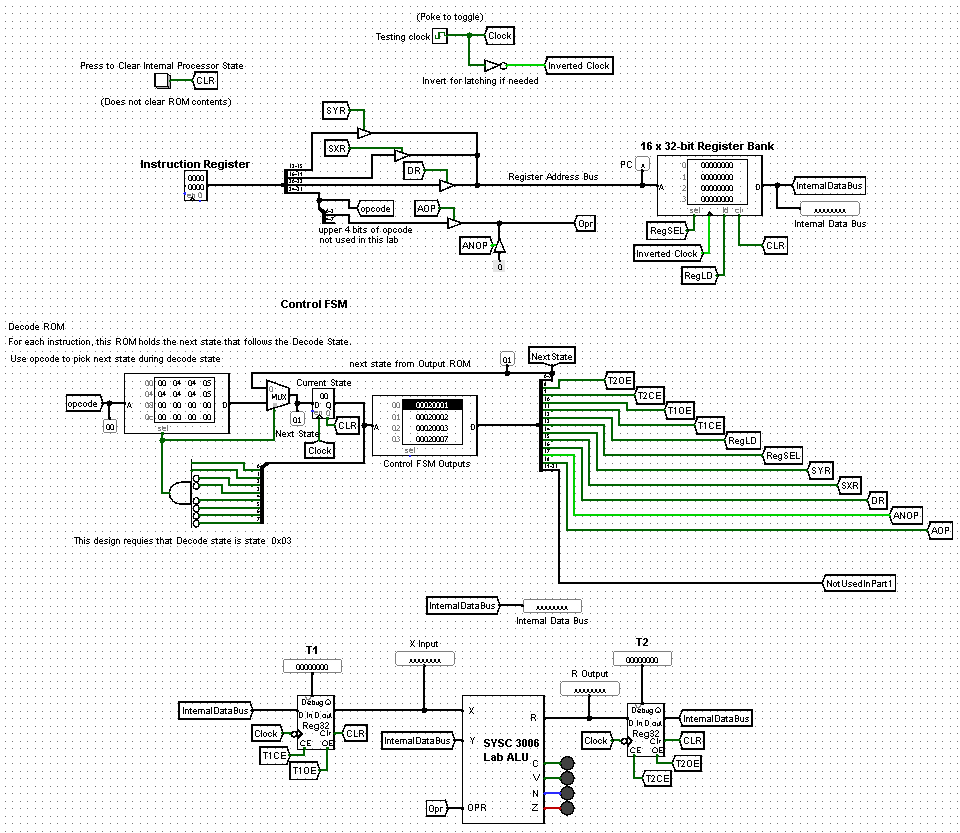
\includegraphics[width=0.72\textheight]{circuit_part1.png}
		\caption{Logisim Circuit of Part 1}
	\end{figure}

	\pagebreak

	\subsection{Same as you did in lab 2, execute the instructions in the table above in the given sequence with all registers initially containing 0x0. Log the execution of the sequence on your implementation to validate the execution of the required instructions and show the results here. (The simulation log should include: Current State, IR, PC, registers, and Next State. Set the log radix to hex).}
	
	\begin{table}[!ht]
		\centering
		\caption{Simulation Log Table of the operation R5 $\leftarrow$ NOT (R4)}
		\vspace{0.2cm}
		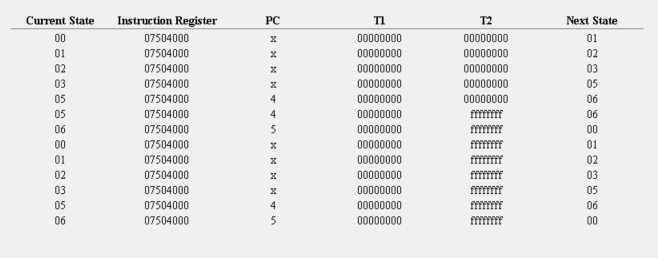
\includegraphics[width=0.9\linewidth]{op07504000.png}		
	\end{table}

	\begin{table}[!ht]
		\centering
		\caption{Simulation Log Table of the operation R7 $\leftarrow$ R6 - R4}
		\vspace{0.2cm}
		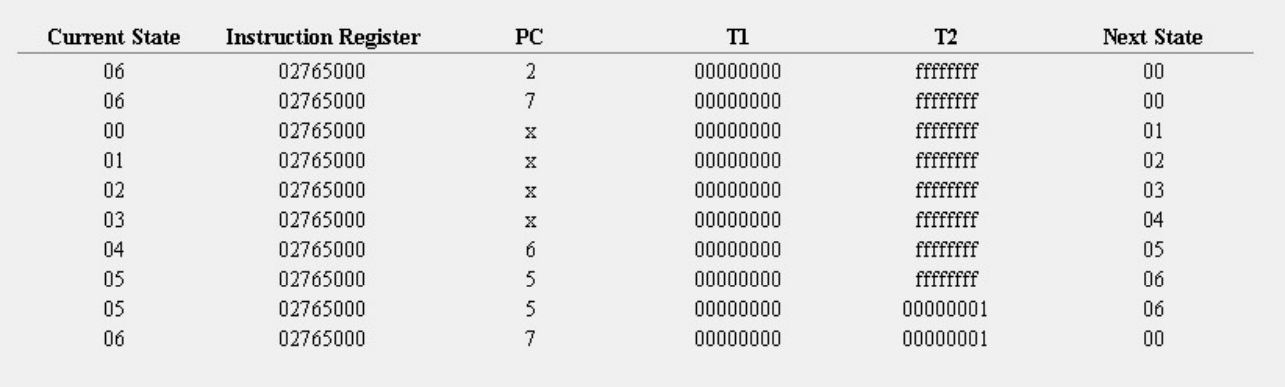
\includegraphics[width=0.9\linewidth]{op02765000.png}	
	\end{table}	

	\pagebreak

	\begin{table}[!ht]
		\centering
		\caption{Simulation Log Table of the operation NOP}
		\vspace{0.2cm}
		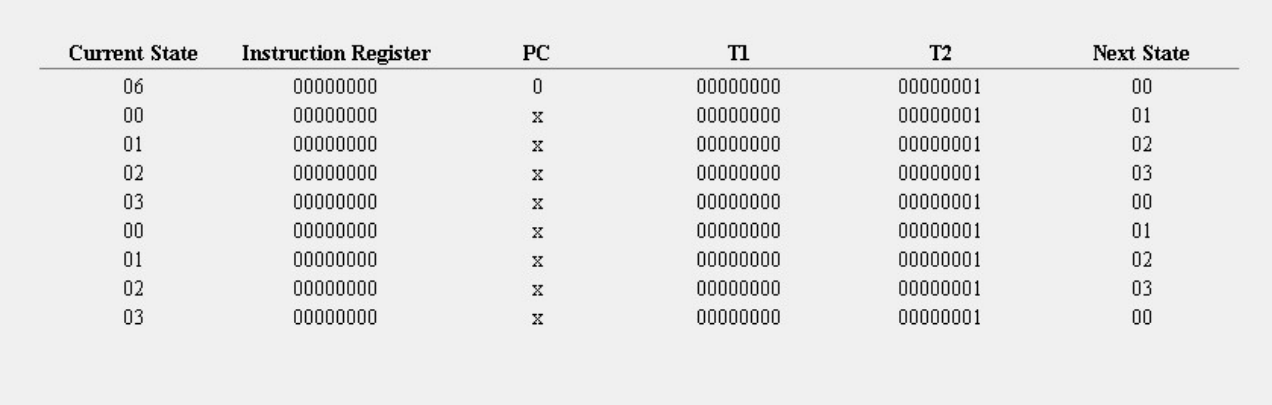
\includegraphics[width=0.9\linewidth]{op00.png}
	\end{table}	

	\begin{table}[!ht]
		\centering
		\caption{Simulation Log Table of the operation R0 $\leftarrow$ R7}
		\vspace{0.2cm}
		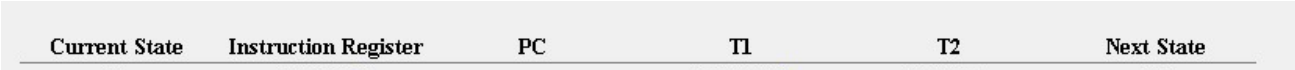
\includegraphics[width=0.9\linewidth]{op03007000_part1.png}
		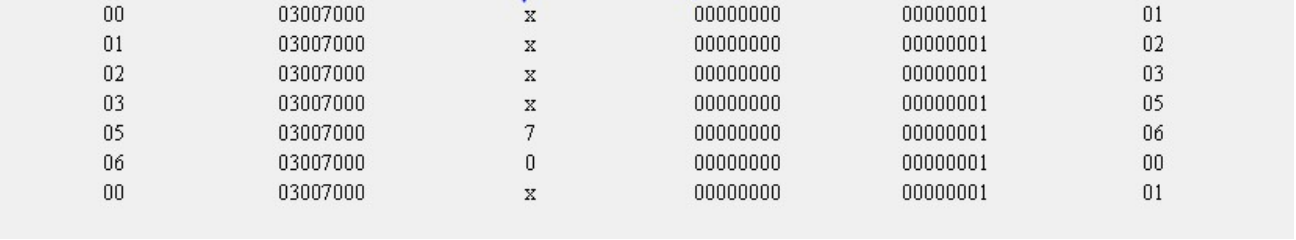
\includegraphics[width=0.9\linewidth]{op03007000_part2.png}	
	\end{table}	
	
	\pagebreak
	
	\section{Second Part}
	\subsection{Tables and Figures}
	\subsubsection{Complete the Part 2 FSM Output ROM Table.}
	\begin{table}[!ht]
		\centering
		\caption{FSM Output ROM for Part 2}
		\vspace{0.2cm}
		\includegraphics[width=0.72\textheight]{fsm_output_part2.png}	
	\end{table}

	\subsubsection{Complete the Part 2 Main Memory Instructions Table for the following instructions.}
	\begin{table}[!ht]
		\centering
		\caption{Main Memory Instruction Table}
		\vspace{0.2cm}
		\begin{tabular}{|c|c|c|}
			\hline
			Instruction & Address (Hex) & Contents (Hex)\\
			\hline\hline
			R10 $\leftarrow$ R1 OR R2 & 00 & 05A1 2000\\
			\hline
			R11 $\leftarrow$ R2 - R10 & 01 & 02B2 A000\\
			\hline
			R12 $\leftarrow$ NOT (R11) & 02 & 07C0 B000\\
			\hline
			R13 $\leftarrow$ R0 + R12 & 03 & 01D0 C000\\
			\hline
		\end{tabular}
	\end{table}

	\pagebreak

	\subsection{Circuit Wiring}
	\subsubsection{Show below a screenshot of the new control FMS outputs that you added in the Logisim circuits, and a short description about each output.}
	\begin{figure}[!ht]
		\centering
		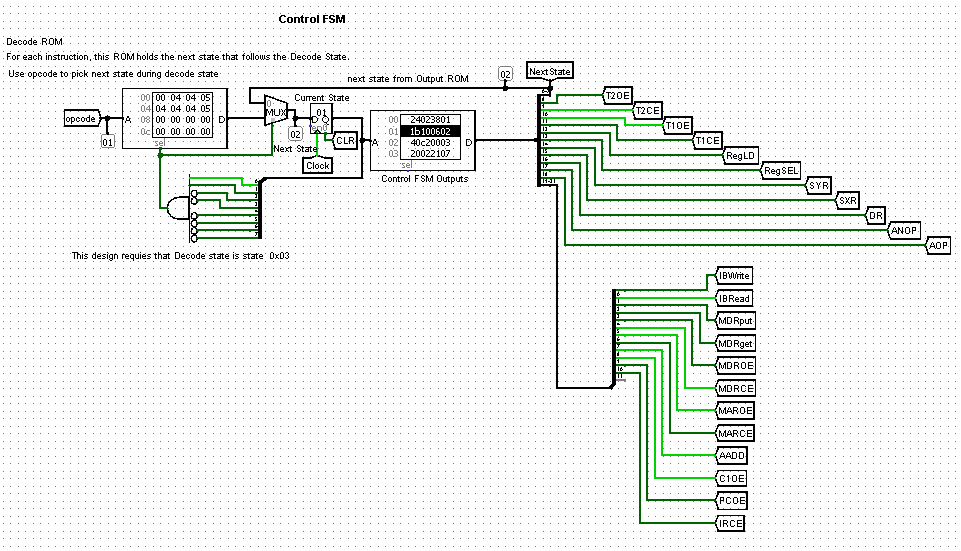
\includegraphics[width=\linewidth]{fsm_circuit_part2}
		\caption{New Control FSM Circuit}
	\end{figure}
	
	\begin{itemize}
		\item IBWrite: allows the register within the interconection bus to be written to
		\item IBRead: allows the register within the interconection bus to be read from
		\item MDRput: hold data exchanged on the interconnection data bus written to main memory
		\item MDRget: hold data exchanged on the interconnection data bus read from main memory
		\item MDROE: determines when the data is outputted from the MDR register
		\item MDRCE: determines when the data is inputted in the MDR register
		\item MAROE: determines when the data is outputted from the MAR register
		\item MARCE: determines when the data is outputted from the MAR register
		\item AADD: provides the ALU with the addition operation
		\item C1OE: inputs 0x00000001 to your internal data bus which then gets added to the PC value
		\item PCOE: introduces new constant to encode the PC's register address (address of R15)
		\item IRCE: introduces signal from internal data bus to the instruction register
	\end{itemize}

	\pagebreak

	\subsubsection{Show here a screenshot of the new hardware components that you added in the Logisim circuits. Include a short description about each component function.}
	\begin{figure}[!ht]
		\centering
		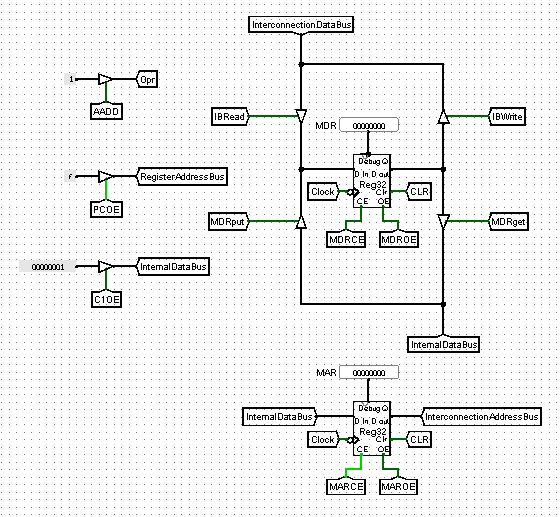
\includegraphics[width=0.7\linewidth]{hardware_added.png}
		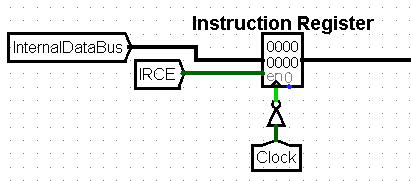
\includegraphics[width=0.5\linewidth]{instruction_register.png}
		\caption{New Hardware Components added to the Logisim Circuit}
	\end{figure}

	A value is inputted from the internal data bus into the MDR and then outputted to the interconnection data bus. A value can also be read from the interconnection data bus to the register and then passed to the internal data bus.\\
	
	The internal data bus goes to the MAR and then passed to the interconnection address bus.
	The register holds the address that is accessed by the interconnection address bus when outputted.\\
	
	AADD provides the ALU with the addition operation which replaces the operation code that is inputted from the instruction register data.
	This allows the ALU to add 1 to the PC value.\\
	
	PCOE introduces new constant to encode the PC's register address (address of R15).
	C1OE inputs 0x00000001 to your internal data bus which then gets added to the PC value.\\

	Connecting IR to the internal data bus and adding IRCE control and Inverted Clock to allow fetching the Instruction from the internal data into IR at the falling edge of the clock.

	\subsubsection{Include a copy of your Lab3-Part-2.circ circuit with your submission. We must verify your circuit functionality in order to assign you marks for this part (c).}
	\begin{figure}[!ht]
		\centering
		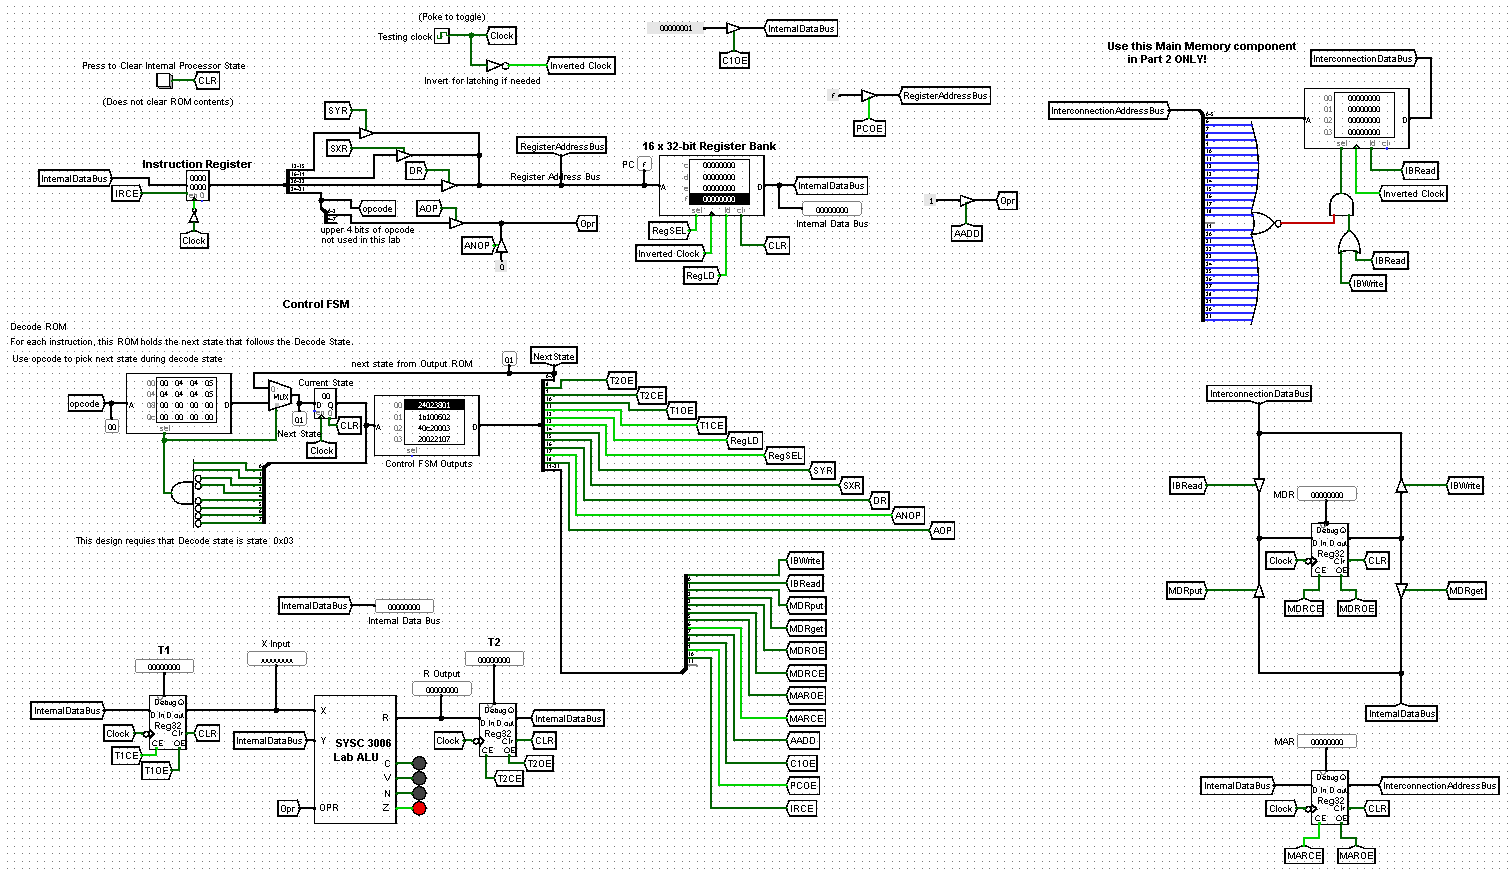
\includegraphics[width=\linewidth]{circuit_part2.png}
		\caption{Logism Circuit of Part 2}
	\end{figure}

	\subsection{Execution Test}
	\subsubsection{Log the execution of the sequence on your implementation to validate the execution of the required instructions and show the results here.}
	\begin{table}[!ht]
		\centering
		\caption{Simulation Log Table of the Part 2 Circuit}
		\vspace{0.2cm}
		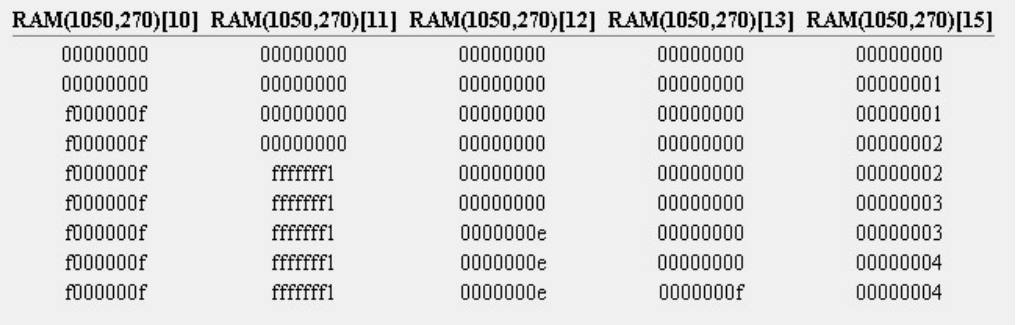
\includegraphics[width=\linewidth]{log_sim_table_part2.png}		
	\end{table}	
	
	\subsubsection{Compare the concept used here to your lab 2-part 2, briefly describe here what is the advantage of the concept here over lab2-part2?}		
	The advantage of this concept is that it allows the user to not change the values in the instruction register.
	The data is read from main memeory and the circuit will automatically performs the instructions on the data.
	This is much quicker to complete the exact same instructions in comparison to lab2-part 2. 
	This setup also allows us to see whenever an operation occurs. 
	Due to the fact that there is a counter at memory location R15, it increments by one every time we go through all the states. 
	This helps to keep track of the total number of operations that have occurred and lets stop at a desired operation. 
\end{document}